\documentclass[aspectratio=43, dvipsnames]{beamer}
\usepackage[version=4]{mhchem}
\usepackage[aboveskip=1pt, belowskip=1pt]{caption}
\usepackage{amsmath}
\usepackage{siunitx}
\usepackage{emoji}
\usepackage{pgfplots}
\pgfplotsset{compat=1.18,}

% Command to display isotopes
\newcommand{\iso}[2]{\ce{^{#1}#2}}
% Command to write overlap
\newcommand{\overlap}[2]{\left\langle#1\middle\vert#2\right\rangle}
% Command to write Rs
\newcommand{\rs}{$\text{R}_{\text{S}}$ }
% Command to draw enumitems outside the environment
\newcommand{\enumitem}[1]{%
\setcounter{enumi}{#1}\usebeamertemplate{enumerate item}% 
}
\newcommand{\boxitem}[1]{\raisebox{0.15em}{\enumitem{#1}}}
% Set caption package options
\captionsetup{labelformat=empty}

\title[Oxygen spectroscopy]{Low-lying spectroscopy of 20O}
\date[Feb 2025]{February 2025}
\author[M. Lozano et al.]{M. Lozano-González, B. Fernández-Domínguez, \texorpdfstring{\newline}{} J. Lois-Fuentes, F. Delaunay}
\institute{USC-IGFAE and LPC-Caen}

\usetheme{igfae}

\begin{document}

\maketitle

\section{Motivation}
\begin{frame}{A recap on spectroscopic factors}
	\textbf{Spectroscopic factors} shed light on the occupancy of single-particle states:
	\begin{equation*}
		\left.\frac{d\sigma}{d\Omega}\right\vert_{\text{exp}} = C^{2}S \cdot \left.\frac{d\sigma}{d\Omega}\right\vert_{\text{s.p}}, \quad \sum C^{2}S = (2j + 1) \text{ in IPSM}
	\end{equation*}
	\begin{columns}[T]
		\begin{column}{0.48\linewidth}
			\hfill{}
			\begin{beamercolorbox}[sep=0.75em, center, wd=0.85\linewidth,rounded=true]{box1}
				\textbf{Experimentally:} Reduction of \sim\qty{65}{\percent}!
			\end{beamercolorbox}%
			\hfill{}
			\begin{itemize}
				\item \textbf{Short-range} correlations: tensor forces,...
				\item \textbf{Long-range}: vibrations, giant resonances,...
			\end{itemize}
		\end{column}
		\begin{column}{0.48\linewidth}
			\vspace{-1em}
			\begin{figure}
				\includegraphics[width=0.725\linewidth]{example-image}
				\caption{L. Lapikás, Nuclear Phys. A 553 (1993)}
			\end{figure}
		\end{column}
	\end{columns}
\end{frame}

\section{Experimental setup}
\begin{frame}{Experimental setup}
	E796 was performed at LISE (GANIL) back in March 2022 under these experimental conditions:
	\begin{columns}[t]
		\begin{column}{0.5\linewidth}
			\begin{itemize}
				\item Beam: \iso{20}{O} @ \qty{35}{A\MeV}
				\item Gas: \qty{90}{\percent}\ce{D_2} and \qty{10}{\percent} \ce{iC_4H_{10}}
				\item Silicons: two front layers and one left. \qty{500}{\micro\m}-thick
			\end{itemize}
			\mycolorbox[0.4]{box2}{
				\textbf{Neutron removal}\\
				$\iso{20}{O}(\iso{}{p}, \iso{}{d})$\\
				$\iso{20}{O}(\iso{}{d}, \iso{}{t})$
			}\hfill
			\mycolorbox[0.4]{box3}{
				\textbf{Proton removal}\\
				$\iso{20}{O}(\iso{}{d},\iso{3}{He})$
			}
		\end{column}\hfil
		\begin{column}{0.45\linewidth}
			\begin{figure}
				\begin{center}
					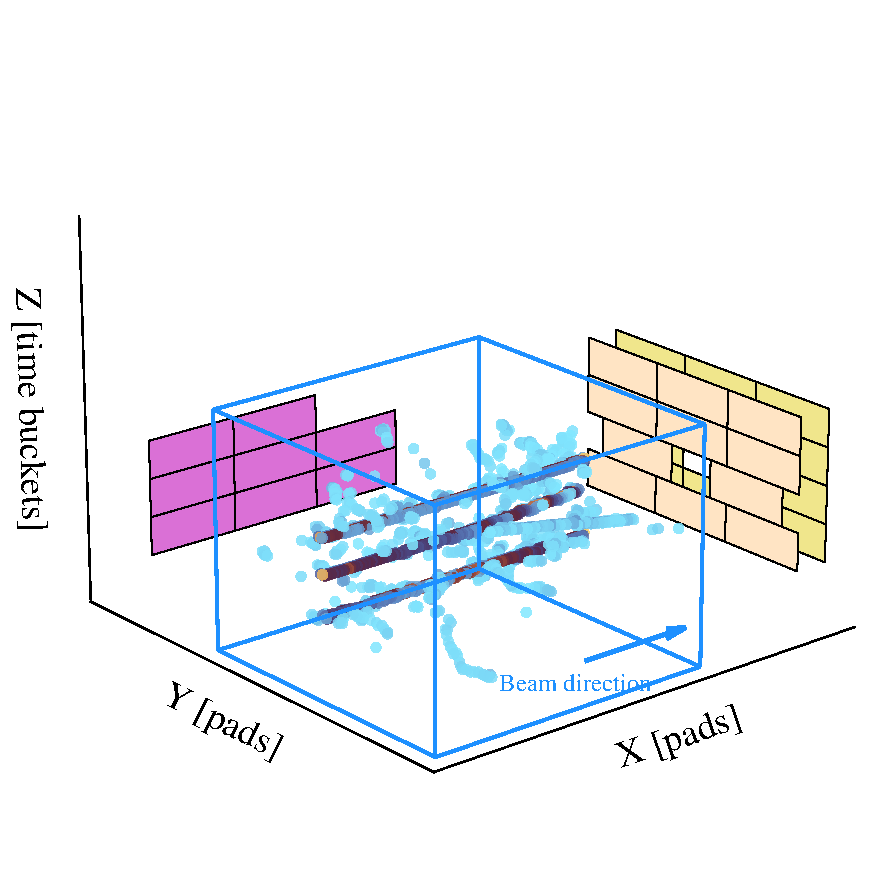
\includegraphics[width=0.95\textwidth]{figures/setup.pdf}
				\end{center}
			\end{figure}

		\end{column}
	\end{columns}

\end{frame}

\section{Results}
\begin{frame}{Results: (in)elastic scattering}
	These are the excitation energy spectra for protons and deuterons.
	\begin{figure}
		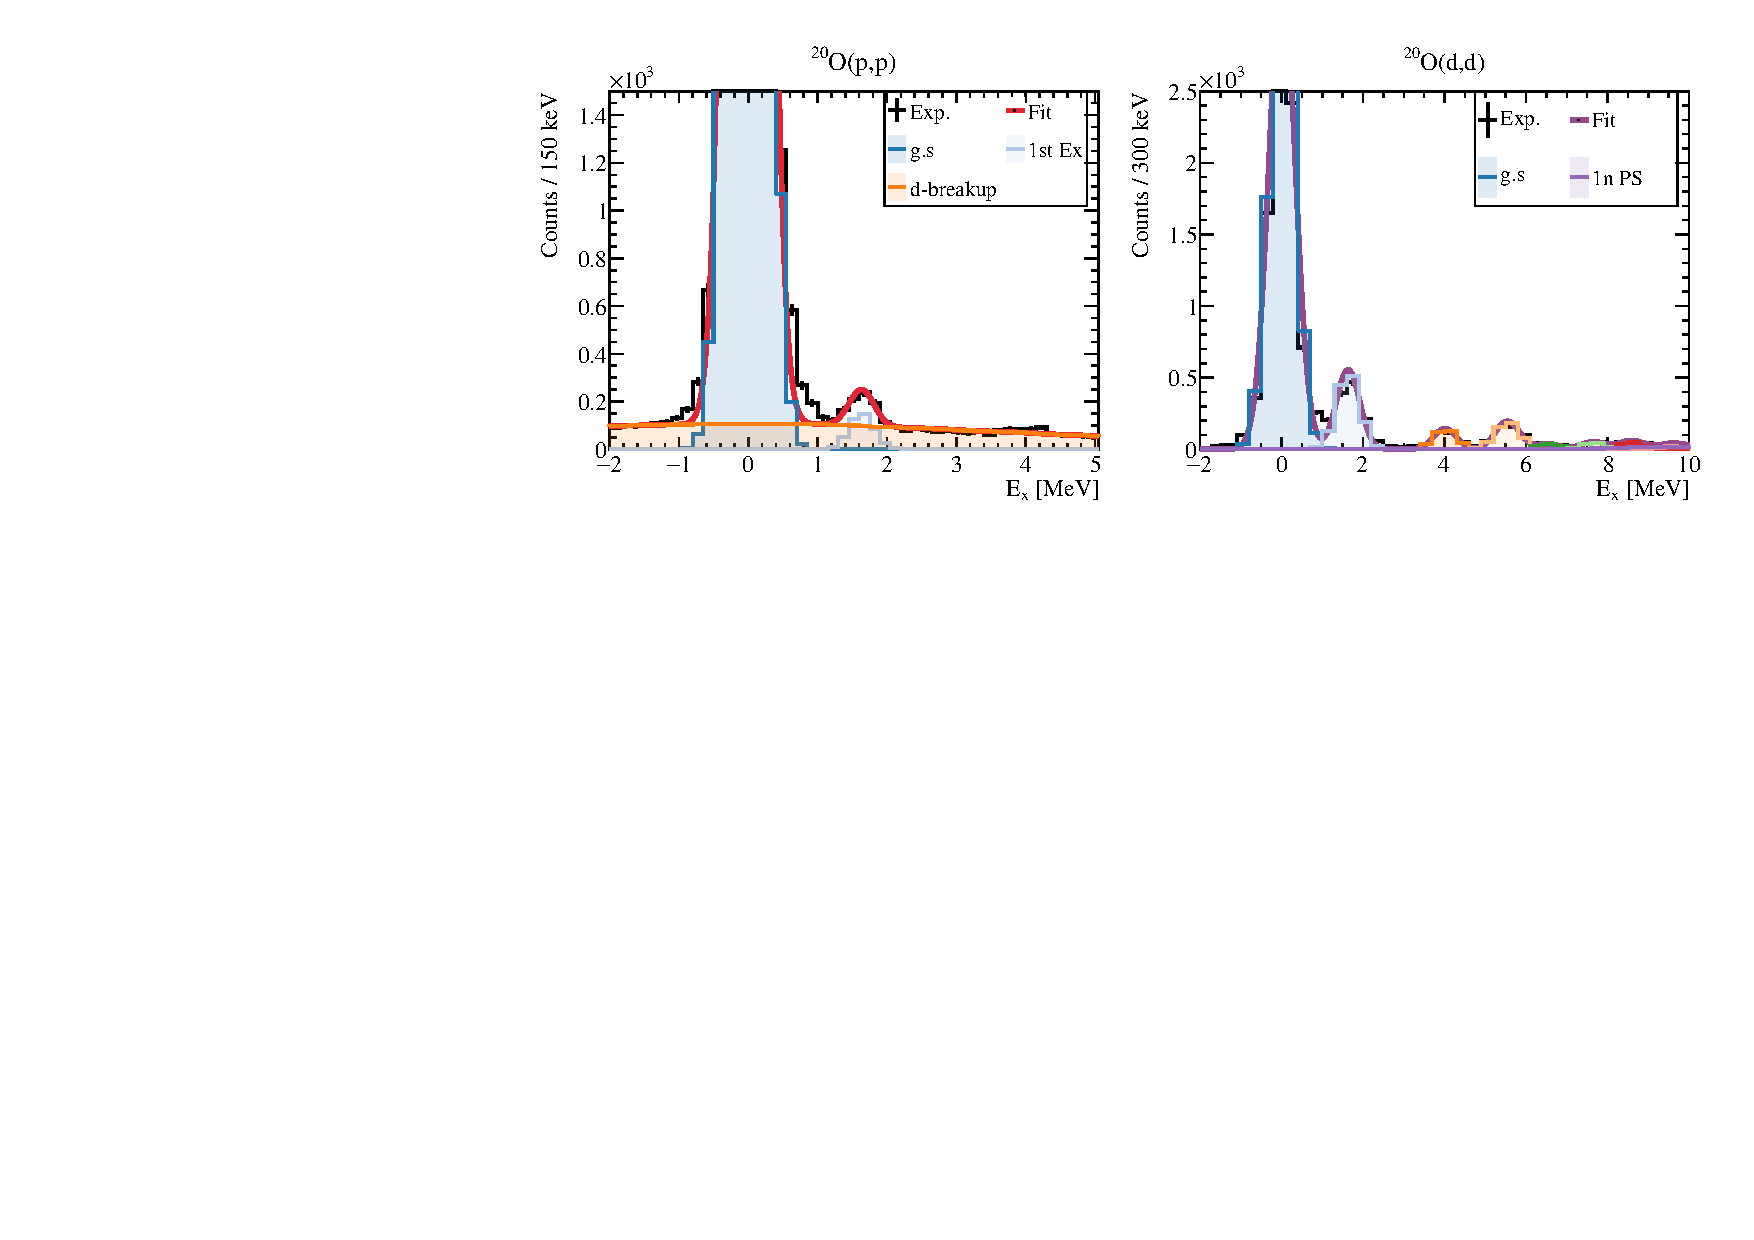
\includegraphics[width=0.95\textwidth]{figures/elastic_xz.pdf}
		% \caption{}
	\end{figure}


\end{frame}



\end{document}
